%!TEX root = thesis.tex

\chapter{Results and Evaluation}
\label{chapter:Results and Evaluation}

This chapter will cover the subsystems and steps taken that were needed to achieve the testing environment described in Chapter~\ref{chapter:Proposed architecture}. This chapter will first discuss the arrangements related to the hardware of the framework and then software related arrangements will be presented and described. After presenting the built framework, achieved results will be discussed and finally the test environment presented in this Thesis will be evaluated.

\section{Hardware arrangements}
\label{section:Hardware arrangements}

\subsection{The Robot}
\label{subsection:Robot}

As suggested in Section \ref{subsection:The Robot proposal}, ShapeOko 2 open-source CNC milling machine was used as robot manipulating the payment terminals. ShapeOko was built according to the instructions found from the homepage of the project (\emph{\cite{shapeoko}}). Construction was altered only regarding to the tool that was used as the spindle motor was substituted by 3D printed pushing tool.

ShapeOko 2 has a working area of about 300 mm x 300 mm x 60 mm and this meas that it can accommodate up to three payment terminals at same time to the working area. This allows parallel test case execution i.e. test cases can be run at the same time with different terminals. Arrangement of the devices was implemented by dividing the work area into three sections. Each payment terminal was attached to a standard sized MDF-plate and each section of the working are can accommodate one of these MDF-plates. Holes were drilled in to the working area and nuts were inserted in to these holes at the back of the work bench. MDF-plates attach to these holes with screws enabling easy installation and removal of plates with different models of payment terminals.

\begin{figure}[ht]
  \begin{center}
    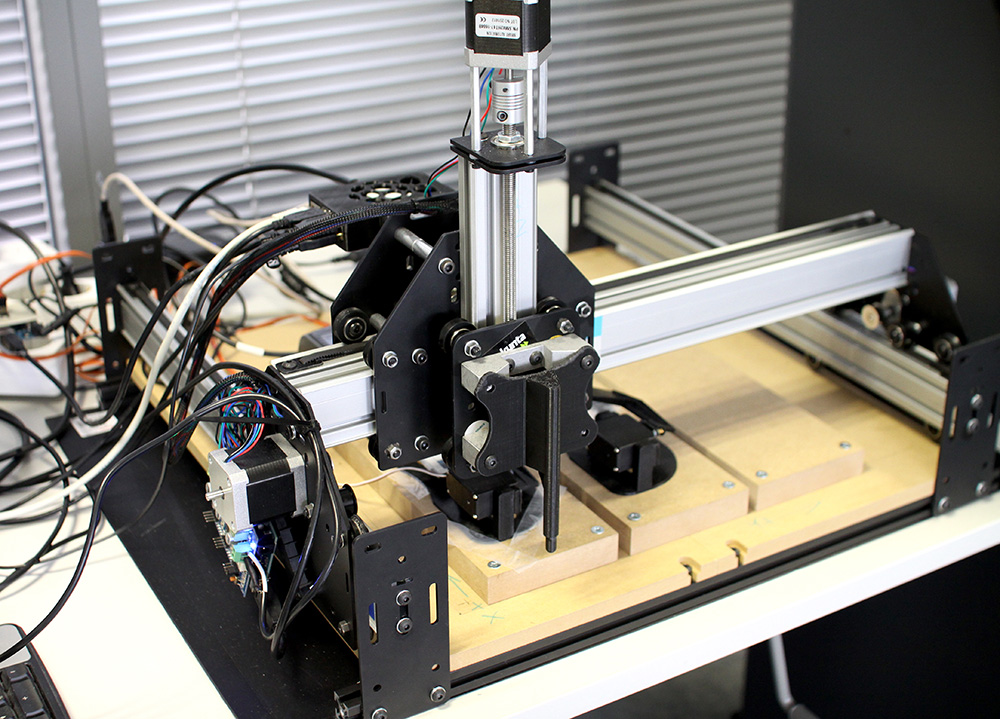
\includegraphics[width=10cm]{images/robot.jpg}
    \caption{Robot in its production state.}
    \label{fig:robot_final}
  \end{center}
\end{figure}
\FloatBarrier

Section \ref{subsection:The Robot proposal} suggests equipping the robot with a pushing tool and this was implemented to the final solution by 3D printing the tool from PLA plastic. Tool consisted of two parts: cylindrical beam and a stem inside of it. Stem slides inside the beam and the two parts are segregated with a spring. Spring provides the needed attenuation when pressing the buttons of the payment terminals. Pushing tool can be observed in Figure \ref{fig:pushing_tool} and Figure \ref{fig:robot_final}.

\begin{figure}[ht]
  \begin{center}
    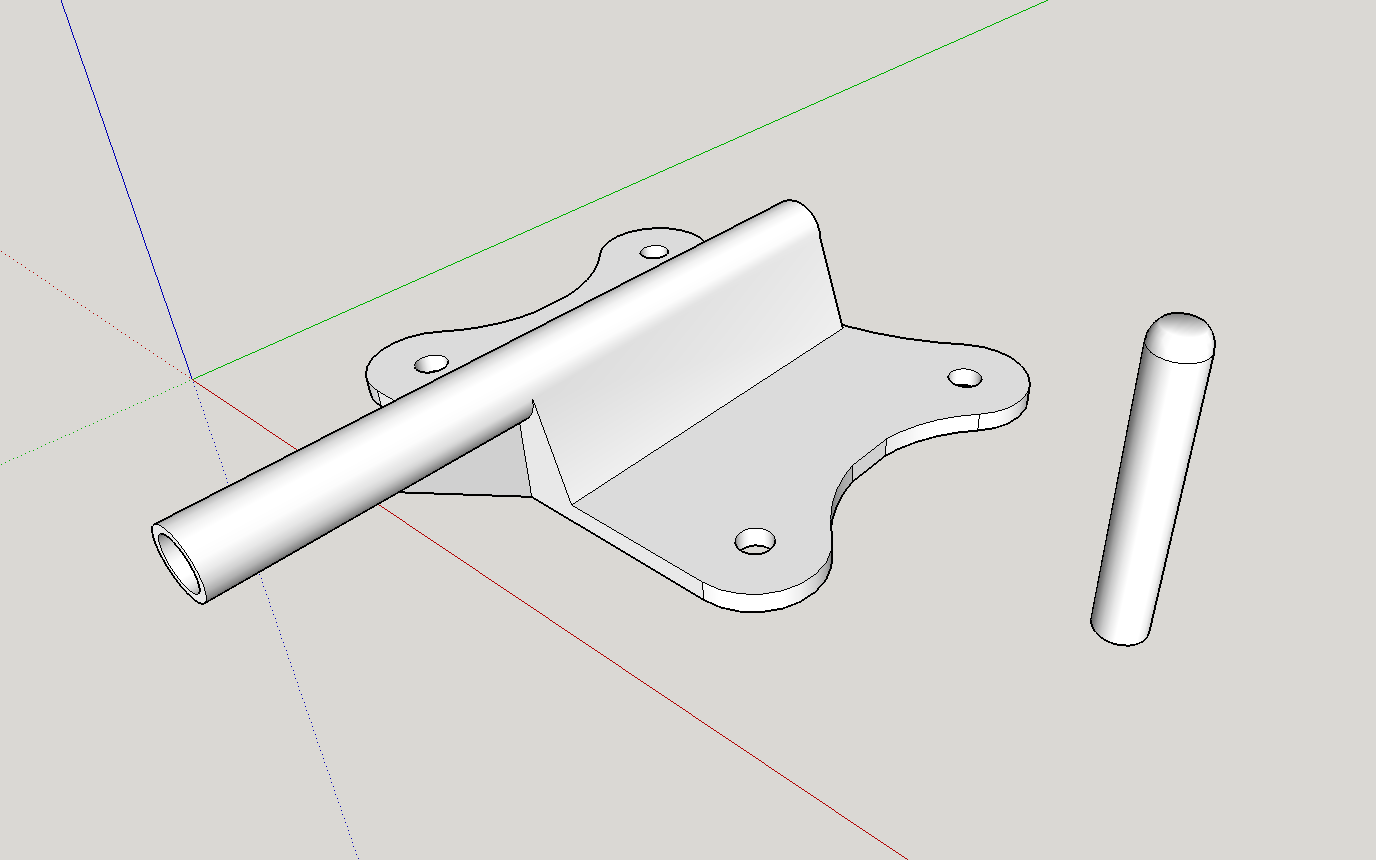
\includegraphics[width=10cm]{images/pushing_tool.png}
    \caption{CAD design of the pushing tool.}
    \label{fig:pushing_tool}
  \end{center}
\end{figure}
\FloatBarrier

\subsection{Computing hardware}
\label{subsection:Computing hardware}

Raspberry Pi 2 Model B single-board computer is used as a main computer of the AAT environment. Raspberry Pi provides optimal computing power compared to it's price and has big community of users and developers world wide. Board is covered with 3D printed enclosure and it is attached to the robot.

In addition to the Raspberry Pi 2, the robot also has two Arduino Uno boards for handling some specific functionalities of the AAT environment. One Arduino Uno is interpreting the G-code commands sent from the Raspberry Pi and it is connected to the stepper motors of the robot through a stepper motor driver shield\footnote{\url{http://www.shapeoko.com/wiki/index.php/GrblShield/}}.

Second Arduino Uno is handling the servo motor control of the card feeders. It is connected to the Raspberry Pi via USB connection and control commands to Arduino Uno are sent using serial communication. Arduino board provides PWM signal to the servo motors and can accommodate three card feeders at the same time. Self-made circuit board was fabricated and attached on top of the Arduino board in order to make connecting the servo motor cables easy.

Connection diagram and main electronic components are visualizes in Figure \ref{fig:electronics}. 

\begin{figure}[ht]
  \begin{center}
    \includegraphics[width=10cm]{images/electronics.png}
    \caption{Main electronic components and connection diagram of the robot. Sources: \emph{\cite{image1}}, \emph{\cite{image2}}, \emph{\cite{image3}}, \emph{\cite{image4}}, \emph{\cite{image5}}}
    \label{fig:electronics}
  \end{center}
\end{figure}
\FloatBarrier

\subsection{Camera arrangements}
\label{subsection:Camera Arrangements}

As suggested in Section \ref{section:Proposed hardware}, Raspberry Pi's own camera module was used for machine vision hardware. Camera was attached to the bottom of the Raspberry Pi's enclosure and the enclosure was attached to the Z-axis assembly of the robot to the opposite side where the pushing tool is. Camera can be moved within the X- and Y-axis. Z-axis movement of the camera isn't possible. Depth of focus of the camera provides clear image of the screen even when the distance between the lens and the screen differs slightly between different payment terminal models. Camera attachment can be seen in Figure \ref{fig:camera}.

\begin{figure}[ht]
  \begin{center}
    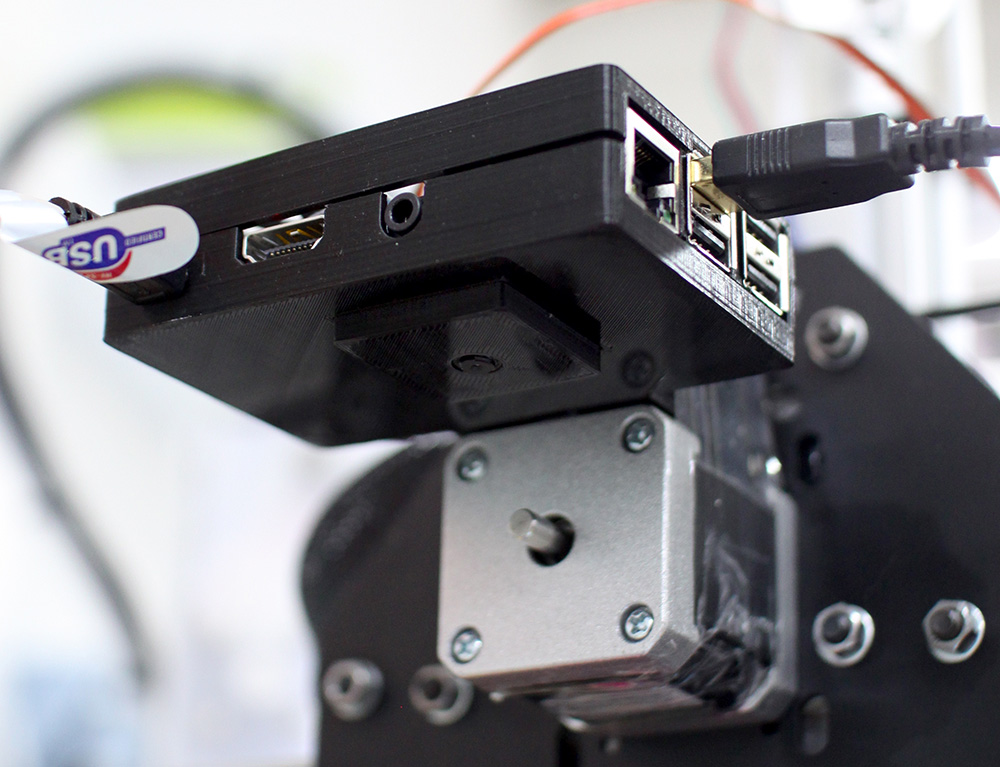
\includegraphics[width=10cm]{images/camera.jpg}
    \caption{Camera is attached to the bottom of the Raspberry Pi's enclosure.}
    \label{fig:camera}
  \end{center}
\end{figure}
\FloatBarrier


\subsection{Card feeder arrangements}
\label{subsection:Card feeder arrangements}

As suggested in Section \ref{subsection:Card feeder}, card feeder frames were 3D printed using PLA plastic. Finalized card feeders consisted of bottom plate, payment card holder and servo motor. Servo motor attaches directly to the bottom plate and card holder attaches to the arm of the servo motor.

Simplistic design can be used with different kinds of payment terminals which have the card slot at the bottom edge of the device. Flexibility provided by the plastic structure and the payment card itself allows the solution to be compatible with most of the payment terminals of this type. Design of the card feeders is presented in Figure \ref{fig:card_feeder}

\begin{figure}[ht]
  \begin{center}
    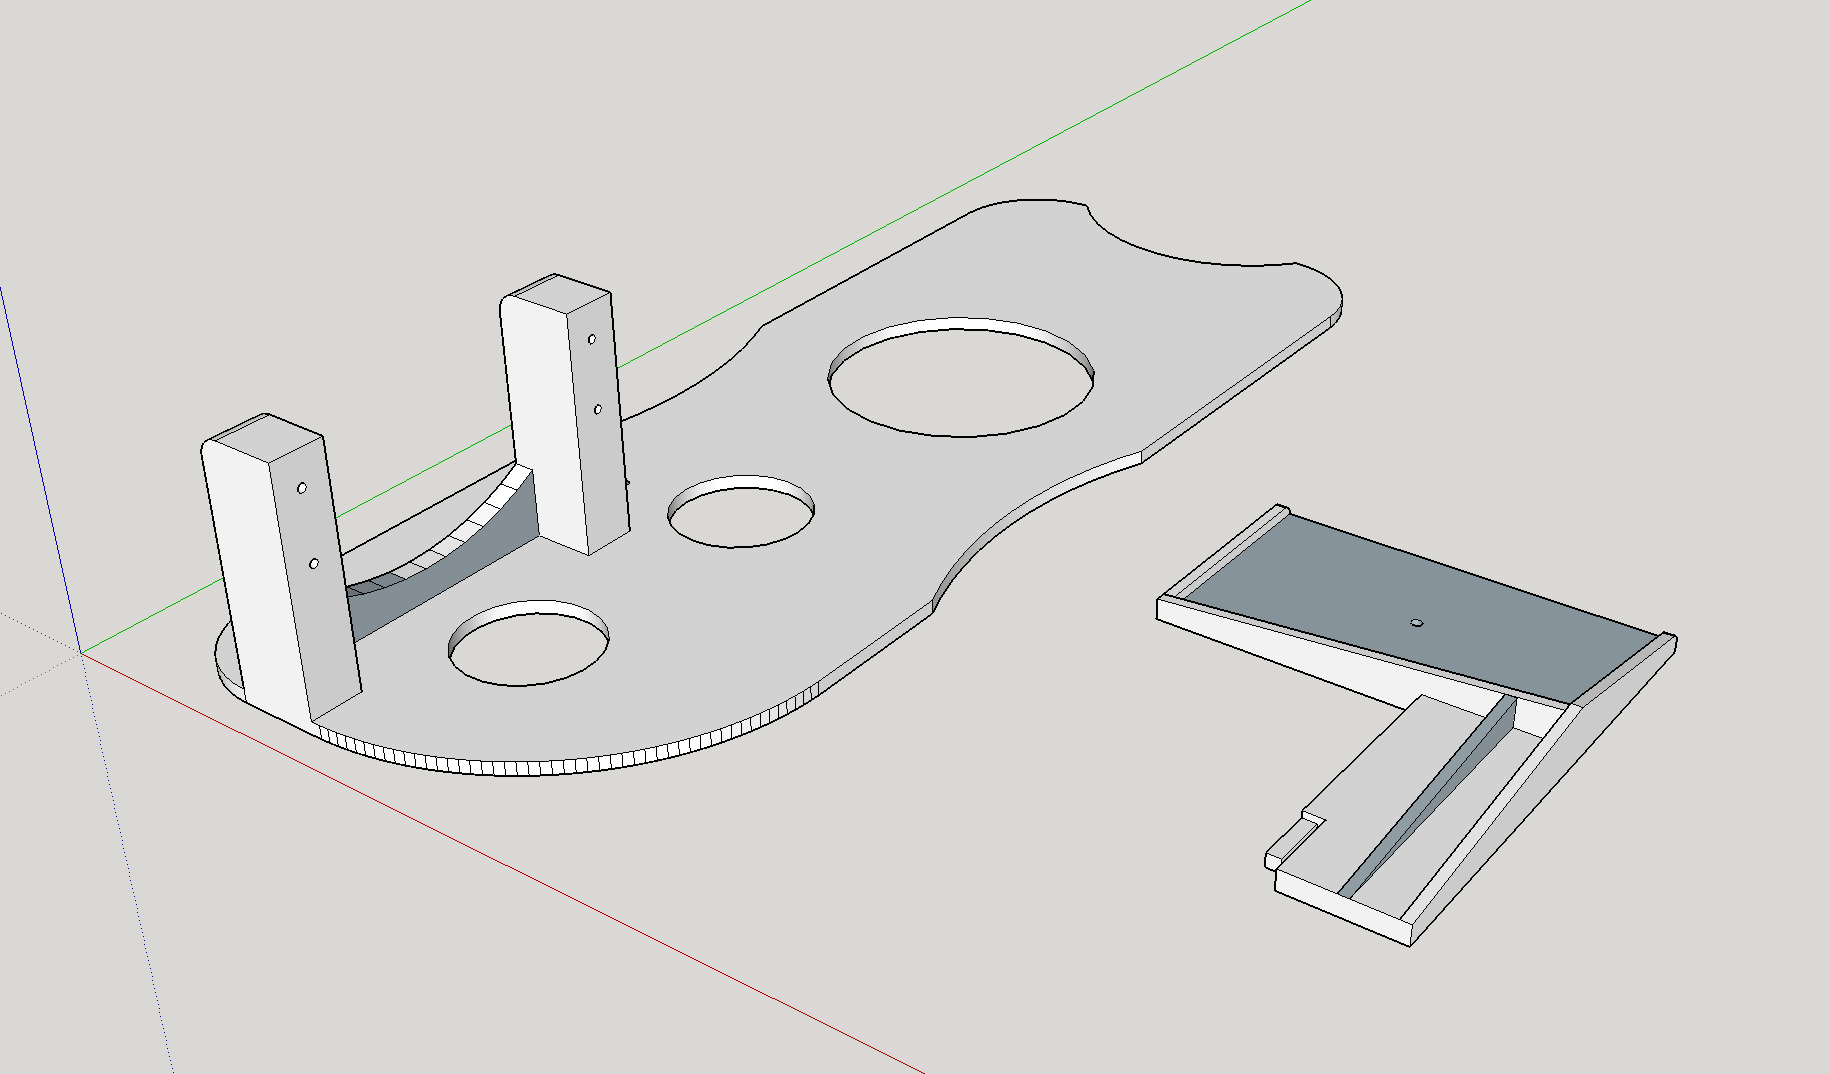
\includegraphics[width=12cm]{images/card_feeder.png}
    \caption{CAD design of the card feeder.}
    \label{fig:card_feeder}
  \end{center}
\end{figure}
\FloatBarrier

\section{Software arrangements}
\label{section:Software arrangements}

\subsection{Software architecture}
\label{subsection:Software architecture}

\subsection{Robot Framework and libraries}
\label{subsection:Robot Framework and libraries}

\subsection{Computer vision arrangements}
\label{subsection:Computer vision arrangements}

\subsection{Test syntax}
\label{subsection:Test syntax}


\section{Results}
\label{section:Results}

\section{Evaluation}
\label{section:Evaluation}